\section{FOXO3 and FOXK2 bind to both overlapping and specific genomic regions}\label{section:foxo3}

\subsection{Validation of FOXO3 ChIP-seq data}

After the discovery that FOXM1gains its own specific binding events by protein-protein interactions with the MMB complex, we next investigated the DNA-binding specificity of two other typical Forkhead proteins: FOXO3 and FOXK2, both of which bind to the canonical Forkhead consensus and are linked to the cell cycle control.

\begin{figure}[!h]
    \centering
    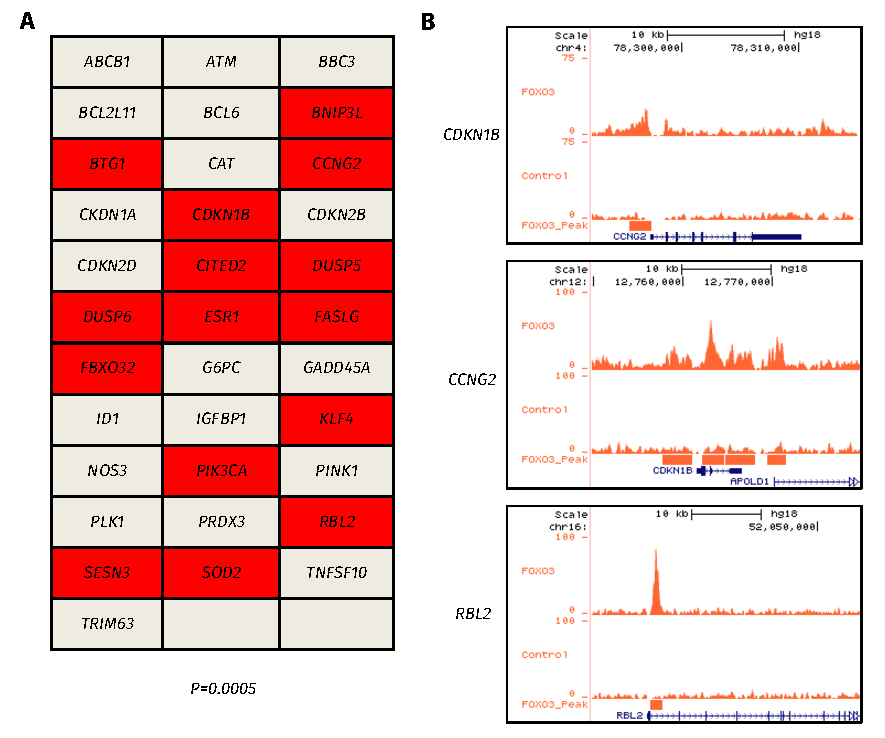
\includegraphics[width=0.9\textwidth]{chapter3/figures_foxo3/fig39.pdf}
    \caption[FOXO3 binding at known target genes]{\textbf{FOXO3 binding at known target genes. (A)} 34 known target genes of FOXO3 according to the transcription factor encyclopaedia (\cite{yusuf2012the}). Red colour indicates the genes that are also identified by the FOXO3 ChIP-seq experiment. The P-value was calculated by a Fisher's exact test. \textbf{(B)} Snapshots of FOXO3 peak profiles at the \textit{CCNG2}, \textit{CDKN1B}, \textit{RBL2} loci.}
    \label{fig:fig39}
\end{figure}

To confirm the reliability of the FOXO3 ChIP-seq experiment, we first checked whether the previously-discovered FOXO3 target genes were actually bound by FOXO3 in the ChIP-seq dataset. Among the 34 manually-curated target genes in The Transcription Factor Encyclopaedia (\cite{yusuf2012the}), 15 of them were bound by FOXO3 (\textbf{Figure \ref{fig:fig39}A}). These include the well-known cell cycle arrest regulators \textit{CCNG2}, \textit{CDKN1B} (\textit{p27}), and \textit{RBL2} (\textit{p130}) (\textbf{Figure \ref{fig:fig39}A} and \textbf{B}). Interestingly, unlike the FOXM1 peaks which are mainly located within the core promoter of its target gene, the locations of FOXO3 peaks around its target genes were quite variable: some were in the promoter region (\textit{e.g. CCNG2}); some were in the gene body (coding exons and introns) (\textit{e.g. RBL2}); some were present in both the promoter and the gene body (\textit{CDKN1B}) (\textbf{Figure \ref{fig:fig39}B}).

Having confirmed that many known FOXO3 target genes are present in the FOXO3 ChIP- seq data, we next started to experimentally validate the ChIP-seq derived FOXO3 peaks. To this end, we randomly selected twelve peaks with varying enrichments from the ChIP-seq data and tested the FOXO3 binding at these loci. ChIP experiments were performed in the U2OS-FOXO3 stable cell line after the treatment with LY294002 to induce FOXO3 nuclear entry and doxycycline to induce FOXO3 expression using the FLAG antibody. All tested regions showed more than 10 fold enrichment over the control ChIP experiments performed in the U2OS T-REX host cell line (\textbf{Figure \ref{fig:fig40}A}). The binding at each locus, as represented by \% input bound, was also positively correlated with the ChIP-seq signal, as represented by the tag density, \textit{i.e.} regions with higher \% input bound tend to have higher tag density according to the ChIP-seq, although this relationship was not linear $R^2=0.48$ (\textbf{Figure \ref{fig:fig40}B}). In addition, the \textit{CCNB1} and \textit{PLK1} promoter regions, where FOXM1 peaks are located, were also included in the experiments as negative control regions. No significant enrichment was detected on either locus (\textbf{Figure \ref{fig:fig40}A}).

\begin{figure}[!h]
    \centering
    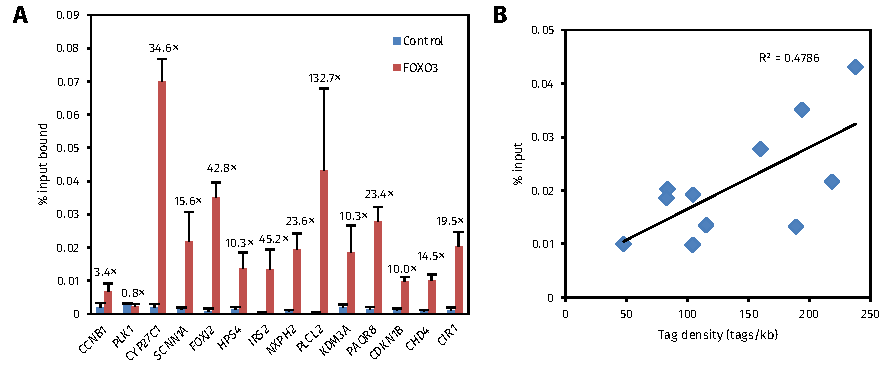
\includegraphics[width=0.9\textwidth]{chapter3/figures_foxo3/fig40.pdf}
    \caption[ChIP-qPCR validation on selected FOXO3 peaks]{\textbf{ChIP-qPCR validation on selected FOXO3 peaks. (A)} Twelve randomly selected FOXO3 peaks with various enrichment levels were tested using ChIP-qPCR. ChIP experiments were performed using a FLAG antibody on the U2OS-FOXO3 stable cell line after 24 hours treatment with doxycycline and 2 hours treatment with LY294002. Fold enrichment over a control ChIP experiment performed on the U2OS T-REX host cell line using the same antibody is indicated above the bar. The error bar represents the standard deviation from three independent experiments. The \textit{CCNB1} and \textit{PLK1} promoter regions, which are bound by FOXM1, were used as negative control regions for FOXO3. \textbf{(B)} Scatter plot of the \% input bound from the ChIP-qPCR and the tag density from the ChIP-seq in the 12 tested regions. The $R^2$ of the trend line was calculated according to a linear regression.}
    \label{fig:fig40}
\end{figure}

Of note, both \textit{CCNB1} and \textit{PLK1} have been shown to be bound by FOXO3 (\cite{alvarez2001forkhead}), indicating its redundant role with FOXM1 on regulating the G2 and M phase cell cycle. However, our ChIP-seq data failed to detect such binding events, and locus-specific ChIP-qPCR demonstrated that FOXO3 does not bind to the \textit{CCNB1} or \textit{PLK1} gene, at least not around their promoters. On the other hand, we still could not rule out the possibility that FOXO3 might bind to the \textit{CCNB1} and \textit{PLK1} genes in certain conditions.

In summary, many known FOXO3 target genes are successfully recovered by our ChIP- seq analysis. Locus-specific ChIP-qPCR shows good enrichments on every tested target and no enrichment on the negative regions. The binding signal from ChIP-qPCR is positively correlated to the ChIP-seq signal. These results indicate that our FOXO3 ChIP- seq data is of good quality.

\subsection{Functional interpretations of FOXO3 binding events}

Having confirmed the quality of the FOXO3 ChIP-seq data, we next investigated whether the FOXO3 peaks define any particular biological processes. To this end, FOXO3 peaks were analysed by GREAT (\cite{mclean2010great}).

Most peaks were assigned to at least one gene, and the majority were assigned to two genes per region (\textbf{Figure \ref{fig:fig41}A}). A total of 5,740 genes were assigned to the 6,089 FOXO3 binding peaks. Fifty-nine peaks were not assigned to any genes, indicating that these regions are located more than 1 megabase from annotated genes. Interestingly, one FOXO3 peak was assigned to 7 different genes (\textbf{Figure \ref{fig:fig41}A}), indicating this peak is located at a region which has a high gene density. Indeed, when looked at the position of this peak (ID: FOXO3\_MACS\_11757), it was located at a region on the chromosome 2 near the \textit{HOXD} gene cluster (data not shown). GREAT returned 16 enriched terms for Biological Process, 6 for Cellular Component, 30 for Mouse Phenotype, and 3 for MSigDB Pathway (\textbf{Figure \ref{fig:fig41}B}).

\begin{figure}[!h]
    \centering
    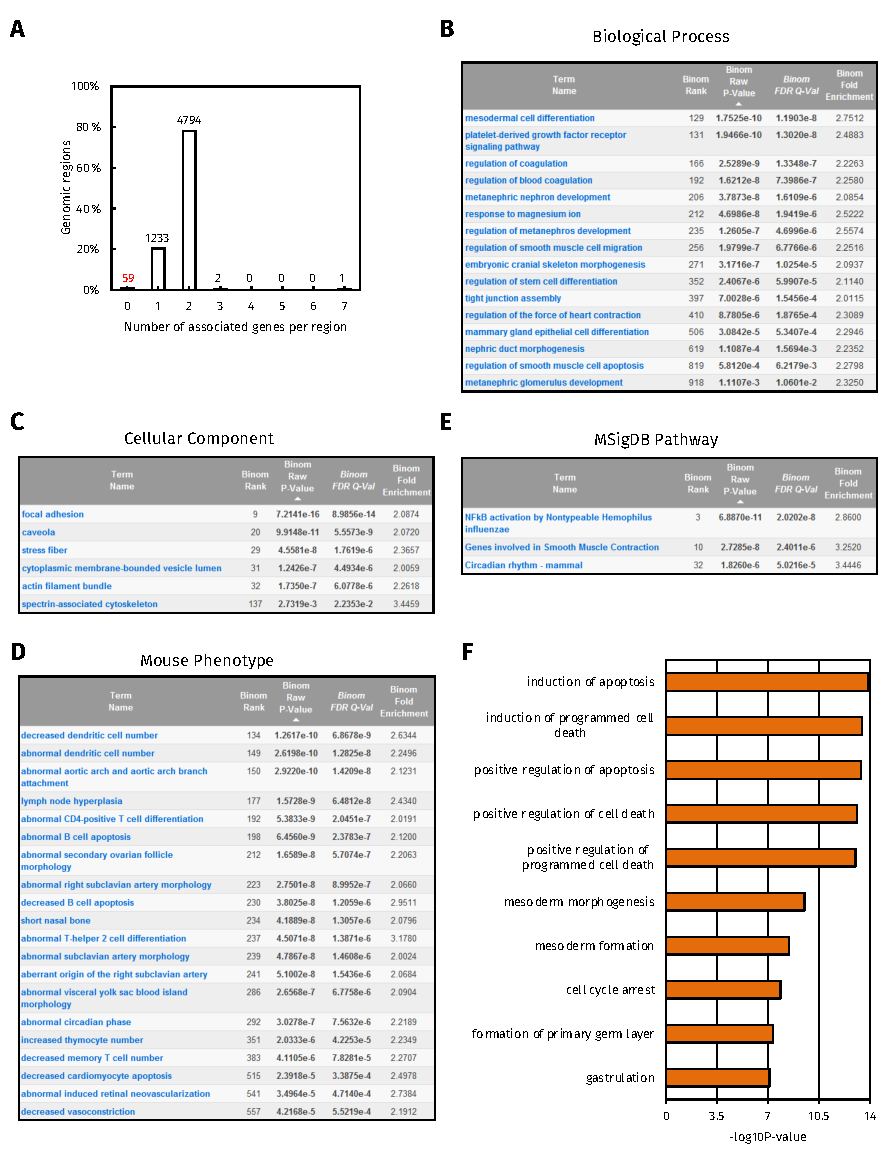
\includegraphics[width=0.9\textwidth]{chapter3/figures_foxo3/fig41.pdf}
    \caption[Gene ontology analysis of FOXO3 peaks by GREAT]{\textbf{Gene ontology analysis of FOXO3 peaks by GREAT. (A)} Histogram showing number of associated genes per peak. (\textbf{B, C, D and E}) GREAT analysis of FOXO3 all peaks (6089). All enriched terms of Biological Process \textbf{(B)}, all enriched terms of Cellular Component \textbf{(C)}, top 20 terms of Mouse Phenotype \textbf{(D)}, and all enriched terms of MSigDB Pathway \textbf{(E)}, were shown. The P-value, FDR, and fold enrichment based on a binomial distribution are also given. \textbf{(F)} Top 10 enriched Biological Process terms of GREAT analysis of FOXO3 top 1000 peaks. The enriched terms were sorted by -$log_{10}$P-value.}
    \label{fig:fig41}
\end{figure}

The top termed returned from the enriched Biological Process was mesodermal cell differentiation, and there were also several other differentiation or development-related terms (\textbf{Figure \ref{fig:fig41}B}). Only recently, FOXO1 and FOXO3 have been identified as essential regulators of the stem cell fate decision in both mouse and human (\cite{renault2009foxo3,zhang2011foxo1}). Our genome-wide analysis of FOXO3 is corroborative to this discovery, which reinforces the discovery that FOXO3 plays a very important role in cell differentiation and development. Interestingly, some other novel functions of FOXO3 were also uncovered, which suggested that FOXO3 regulates the processes involved in coagulation and muscle cell functions (\textbf{Figure \ref{fig:fig41}B}).

The enriched Cellular Component terms were related to adhesion, actin or cytoskeleton (\textbf{Figure \ref{fig:fig41}C}), indicating the FOXO3 target genes are important for providing the mechanical support for cells.

Many enriched Mouse Phenotype terms were related to the apoptosis or differentiation of B and T lymphocytes functions (\textbf{Figure \ref{fig:fig41}D}), indicating that FOXO3 is critical for the immune system by regulating lymphocytes development. Recent studies have shown that FOXO1 is one of the key players in the regulatory network that controls both B and T lymphocytes' functions (\cite{kerdiles2010foxo,lin2010a,ochiai2012a}). Our FOXO3 genomic data strongly suggests that FOXO3 is also involved in the immune system functions, and is likely to function as a redundant factor of FOXO1. Although no direct evidence has demonstrated that FOXO3 controls lymphocyte functions so far, one recent study showed that in the absence of Foxo3, the developmental defects of T regulatory cells caused by the loss of Foxo1 were exacerbated (\cite{kerdiles2010foxo}). Interestingly, the Forkhead transcription factor FOXP3 has long been shown as a key player in T regulatory cells development (\cite{hori2003control}), indicating that FOXOs and FOXPs might form a \enquote{Forkhead code} to regulate lymphocytes' function and development.

The enriched terms returned from MSigDB Pathway indicated that FOXO3 controls the smooth muscle contraction, the activation of the transcription factor NF-$\kappa$B, and the circadian rhythm (\textbf{Figure \ref{fig:fig41}E}), which are consistent with the enriched terms of Biological Process and previous research (\cite{li2012forkhead,zheng2007foxo}).

Having explored the biological functions of the FOXO3 binding events, we did notice that some known functions of FOXO3, like inducing cell cycle arrest and promoting apoptosis, were not unravelled by the gene ontology analysis. However, when the FOXO3 top 1000 peaks (ranked by FDR and fold enrichment from MACS) were put into GREAT to perform the analysis, both cell cycle arrest- and apoptosis-related terms were found significantly enriched in Biological Process (\textbf{Figure \ref{fig:fig41}F}). Indeed, within the top ten most enriched terms, seven of them were about cell cycle arrest and apoptosis, which is consistent with the known functions of FOXO3. GREAT returned 79 enriched terms of Biological Process for the FOXO3 top 1000 peaks, which is much more than the number of enriched terms for the FOXO3 all peaks. Interestingly, the differentiation- and development-related terms were also enriched in the FOXO3 top 1000 peaks (\textbf{Supplementary Table 2}), though not as significant as terms about the cell cycle arrest and the apoptosis.

In summary, the gene ontology analysis recovered many known functions of FOXO3, such as process involved in cell differentiation and development, cell cycle, and apoptosis. The cell cycle arrest- and apoptosis-related genes seem more enriched within the FOXO3 peaks with high binding signals (top 1000). In addition, novel functions of FOXO3 which are related to coagulation and muscle cell contraction were also indicated by the analysis, and further experiments need to be performed to validate the reliability of the new discoveries.

\subsection{Characterisations of the specific and the shared binding events of FOXO3 and FOXK2}

Having confirmed the biological functions of FOXO3, we next focused the analysis on the binding specificities of FOXO3 and FOXK2.

To find out the shared and specific binding events for FOXO3 and FOXK2, their ChIP-seq derived peaks were compared. The number of binding sites between FOXK2 and FOXO3 was quite different. FOXK2 held \textasciitilde 5 times as many binding sites as FOXO3 (\textbf{Figure \ref{fig:fig42}A}). According to the RNA-seq data from The Human Protein Atlas (\cite{uhlen2010towards}), FOXK2 was significantly more abundant (\textasciitilde 30 fold) than FOXO3 in U2OS cells according to their mRNA levels (\textbf{Figure \ref{fig:fig42}B}). Therefore, it is possible that the protein level of FOXK2 is higher than FOXO3 as well. Since factor abundance is important in ChIP-seq experiments, it is tempting to consider the difference of number of binding events as a result of different factor abundance.

\begin{figure}[!h]
    \centering
    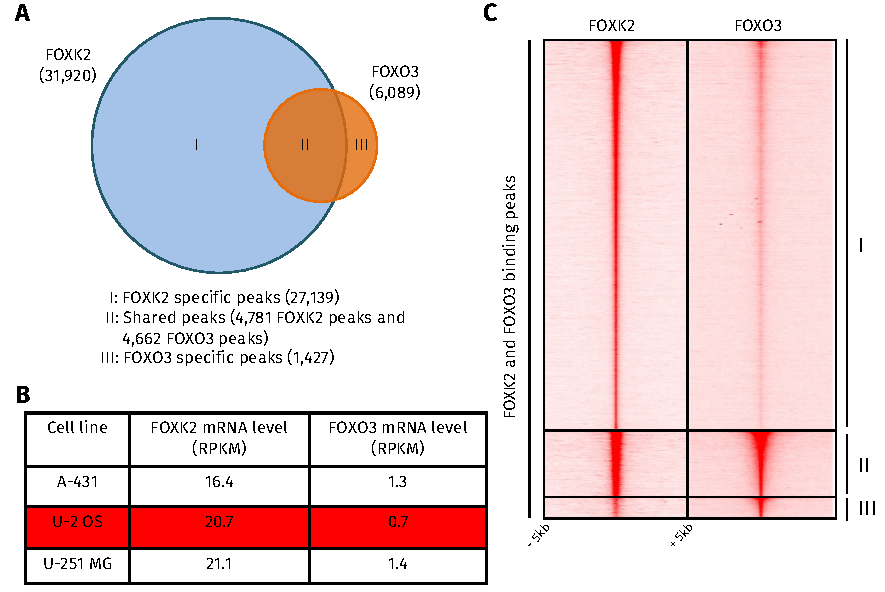
\includegraphics[width=0.9\textwidth]{chapter3/figures_foxo3/fig42.pdf}
    \caption[The overlap of FOXK2 and FOXO3 binding peaks]{\textbf{The overlap of FOXK2 and FOXO3 binding peaks. (A)} Venn diagram showing the overlap of the peaks for FOXO3 and FOXK2. The number of total peaks for each factor and the numbers of FOXK2-specific peaks (I), shared peaks (II) and FOXO3-specific peaks (III) are shown. \textbf{(B)} Quantification of the mRNA levels of FOXK2 and FOXO3 in the indicated cell line. Data was from the RNA-seq experiment in The Human Protein Atlas project (\cite{uhlen2010towards}). Expression values (RPKM, \underline{R}eads \underline{P}er \underline{K}ilobase of exon model per \underline{M}illion mapped reads) from U2OS cells are highlighted. \textbf{(C)} Heatmap of tag density profiles of FOXK2 and FOXO3 around the peaks from the class I, II and III shown in \textbf{(A)}. Peaks in I and II were aligned by the FOXK2 summits, and peaks in III were aligned by the FOXO3 summits. Tags were calculated in every 50 bp bin, and the density profiles were normalised to tags per 10 million total reads per bin. The middle point of each panel (indicated by small arrows below) represents the summit of the peak. 5 kb upstream and 5 kb downstream around the summit were plotted.}
    \label{fig:fig42}
\end{figure}

Since FOXO3 and FOXK2 belong to the same transcription factor family, both shared and specific binding was expected, like members within ETS transcription factor family (\cite{hollenhorst2001mechanisms,wei2010genome-wide}). Here, we define the shared peak as one where peaks overlap by at least one base pair. Indeed, the majority of FOXO3 peaks (~78\%) overlap with FOXK2, and only a small proportion of FOXO3 peaks were specific (\textbf{Figure \ref{fig:fig42}A}). When looking at the sequencing tags around the summit of the specific and shared peaks, there were some FOXO3 binding signals around the summits of FOXK2-specific peaks and vice versa (\textbf{Figure \ref{fig:fig42}C}), but those signals were probably below the threshold used by the MACS or HOMER peak caller. Intriguingly, when the average binding signals of FOXK2 and FOXO3 were compared around the specific and the shared peaks, both factors behaved in a similar way: both of them possessed higher binding signals around the shared peaks than their own specific peaks (\textbf{Figure \ref{fig:fig43}A}). This effect was more prominent in the FOXK2 case (\textbf{Figure \ref{fig:fig43}A}, left panel). The difference of binding signals between the shared and the specific peaks suggests that when binding to the shared regions, both FOXK2 and FOXO3 tend to have higher occupancy. On the other hand, the higher signal intensities within the redundant binding sites could be simply because they are located within open chromatin regions.

\begin{figure}[!h]
    \centering
    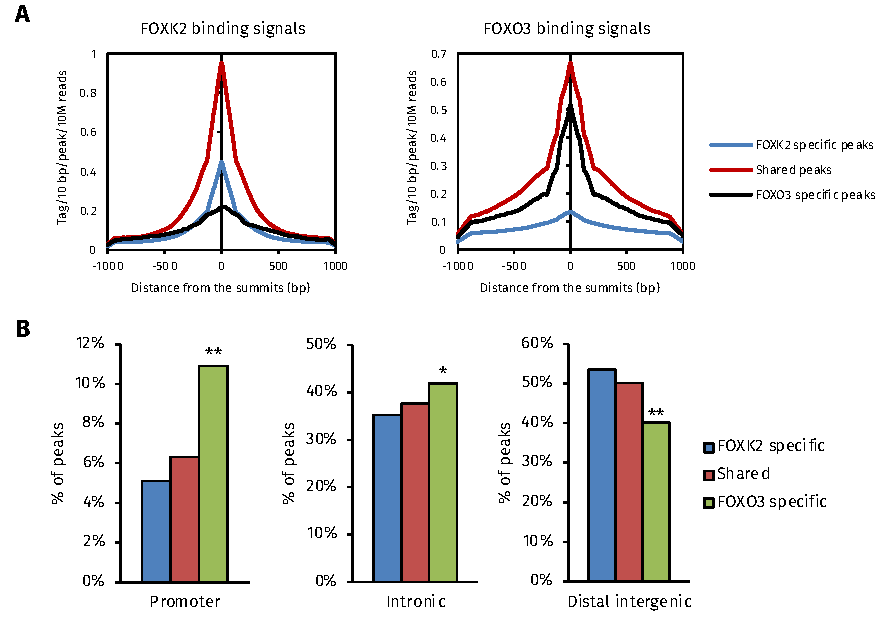
\includegraphics[width=0.9\textwidth]{chapter3/figures_foxo3/fig43.pdf}
    \caption[Tag intensities and genomic distributions of the specific and the shared binding peaks of FOXK2 and FOXO3]{\textbf{Tag intensities and genomic distributions of the specific and the shared binding peaks of FOXK2 and FOXO3. (A)} Quantification of average of tags of FOXK2 (left) and FOXO3 (right) around the summit of indicated peaks. Peaks were aligned by their summits, and a region of -1 and +1 kb relative to the summit was selected. Tags were calculated in every 10 bp bin and normalised to tags per 10 million total reads per bin per peak. \textbf{(B)} Genomic distributions of the indicated peaks. The promoter was defined as 5'-UTR and up to 1 kb upstream from a transcription start site. The distal intergenic region was defined as at least 3 kb upstream from a TSS or at least 3 kb downstream from a TTS. * and ** represent $P<0.005$ and $P<0.0001$, respectively, chi-square test.}
    \label{fig:fig43}
\end{figure}

To further characterise the features of the specific and the shared peaks of FOXK2 and FOXO3, CEAS analysis was performed to check the genomic distribution of the peaks of these three categories. The distributions of the FOXK2-specific peaks and the shared peaks were generally similar, but the FOXO3-specific peaks were more frequently observed within the promoter and the intronic regions and less frequently in the distal intergenic regions (\textbf{Figure \ref{fig:fig43}B}). This indicates that FOXO3, when binding alone, has a different preference towards the promoter and the intronic regions comparing to FOXK2.

Enriched motifs within the peaks often reflect DNA sequence bound by the investigated factor or its interaction partners, and the protein-protein interaction partners often help the factor gain its binding specificity relative to other family members. For example, in budding yeast, Mcm1p interacts with Fkh2p, which helps Fkh2p obtain its specific binding relative to Fkh1p (\cite{hollenhorst2001mechanisms}). Therefore, to further investigate how FOXK2 and FOXO3 obtain their redundant and specific binding sites, \textit{de novo} motif discovery was carried out using HOMER within the 200 bp region centred on the summits of FOXK2 and FOXO3 peaks respectively. The top motifs returned from either FOXK2 or FOXO3 peaks are both Forkhead-like responsive elements, containing the core consensus GTAAACA (\textbf{Figure \ref{fig:fig44}A}). Interestingly, the Forkhead-like responsive elements discovered from FOXK2 and FOXO3 peaks were slightly different: there were some variations not only within the nucleotides in the core consensus and but also in those that are flanking the core consensus (\textbf{Figure \ref{fig:fig44}B}). Generally, the core consensus GTAAACA was the most frequent motif in both FOXK2 and FOXO3 peaks, but A, C, and T at the positions +1, +3, and +6 respectively within the core sequence occurred more frequently in the FOXK2 peaks (\textbf{Figure \ref{fig:fig44}B}). At the flanking regions, there was an overrepresented A or T at the -1 position in both FOXK2 and FOXO3 peaks (\textbf{Figure \ref{fig:fig44}B}), but a G or C was more frequent at the +9 position only in the FOXK2 cistrome (\textbf{Figure \ref{fig:fig44}B}).

\begin{figure}[!h]
    \centering
    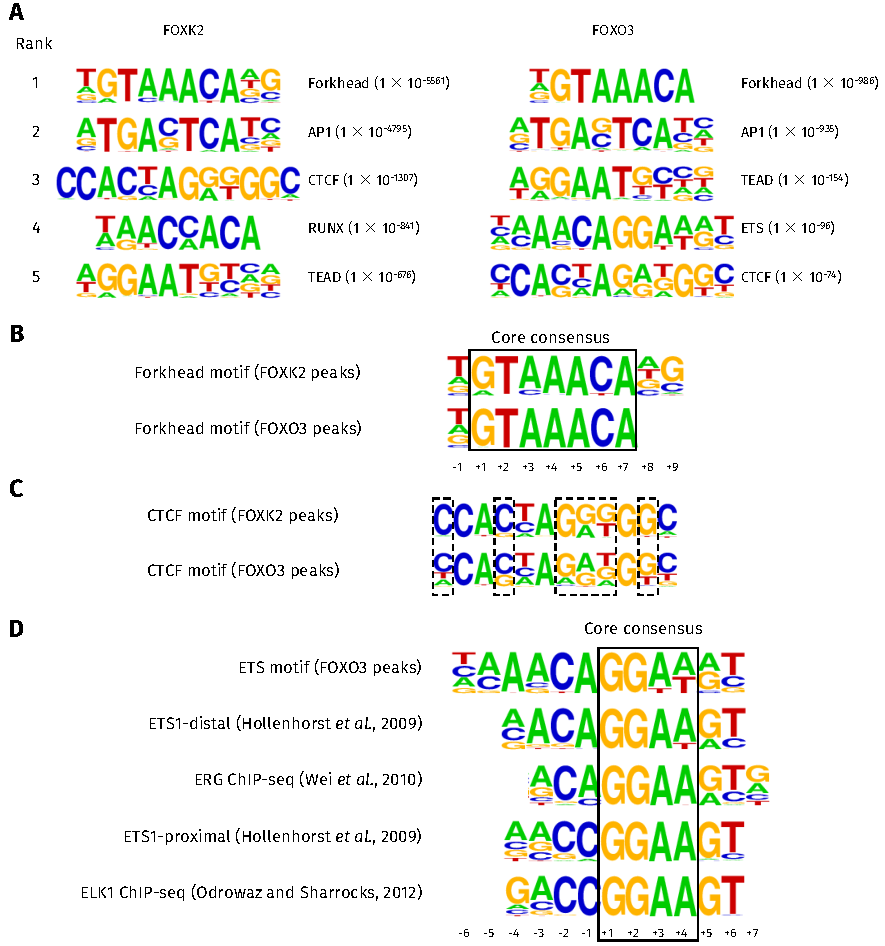
\includegraphics[width=0.9\textwidth]{chapter3/figures_foxo3/fig44.pdf}
    \caption[Overrepresented DNA motifs from FOXK2 and FOXO3 binding peaks]{\textbf{Overrepresented DNA motifs from FOXK2 and FOXO3 binding peaks. (A)} The enriched DNA motifs from FOXK2 and FOXO3 peaks respectively. Motifs are ranked by their P-values which are indicated in parentheses. \textbf{(B)} The comparison of Forkhead motifs returned from the FOXK2 peaks and the FOXO3 peaks. Motifs were aligned to the 5' end of the GTAAACA core sequence, which is highlighted by the rectangle. \textbf{(C)} The comparison of the CTCF motifs returned from the FOXK2 peaks and the FOXO3 peaks. Dotted rectangle highlights the positions which hold higher information content in the CTCF motif from the FOXK2 peaks. \textbf{(D)} The comparison of the ETS motif from the FOXO3 peaks with motifs from ETS1, ERG and ELK1 ChIP-seq. Motifs were aligned to the 5' of the GGAA core sequence which is highlighted by the rectangle.}
    \label{fig:fig44}
\end{figure}

In addition to the Forkhead-like responsive elements, the AP1 motif, the CTCF motif, and the TEAD motif were also found overrepresented within both FOXK2 and FOXO3 peaks, but the RUNX motif and the ETS motifs were only enriched in FOXK2 and FOXO3 peaks respectively (\textbf{Figure \ref{fig:fig44}A}). The AP1 motif and the TEAD motif from the FOXK2 peaks are essentially the same as those from the FOXO3 peaks, but the CTCF motif enriched in the FOXK2 peaks possessed higher information content (stronger motif) than that enriched in the FOXO3 peaks (\textbf{Figure \ref{fig:fig44}C}), suggesting that the CTCF motif might be more overrepresented within the FOXK2 cistrome. The ETS motif from FOXO3 peaks resembled the motifs enriched within the ETS1 distal binding peaks (\textbf{Figure \ref{fig:fig44}D}), but differed from motifs enriched within ETS proximal binding peaks, the ERG binding regions or the ELK1 cistrome (\textbf{Figure \ref{fig:fig44}D}), indicating that FOXO3 might cooperate with specific ETS factors to regulate transcription.

In summary, the numbers of binding sites of FOXK2 and FOXO3 are quite different. FOXK2 has about \textasciitilde 5 times as many binding sites as FOXO3 does. These two factors possess both shared and specific binding regions, and the majority (\textasciitilde 78\%) of FOXO3 binding events are also bound by FOXK2. Such a great extent of overlap between the binding sites of these two proteins is quite unexpected, because previous studies do not suggest any functional redundancy between FOXK2 and FOXO3 (\cite{brunet1999akt,marais2010cell,ji2012the}). The FOXO3 specific binding events are more enriched in the promoter and intronic regions, but occur less frequently within distal intergenic regions. Forkhead-like motifs containing the core sequence GTAAACA are enriched within both FOXK2 and FOXO3 binding event, though there are some sequence variances between the two Forkhead-like motifs. Other transcription factor binding motifs are also enriched within the FOXK2 and the FOXO3 cistromes, indicating the interactions with other transcription factors might help them gain their specific binding events.

\subsection{Nucleotides flanking the Forkhead core consensus are important for the FOXK2 DNA binding both \textit{in vivo} and \textit{in vitro}}

\begin{figure}[!ht]
    \centering
    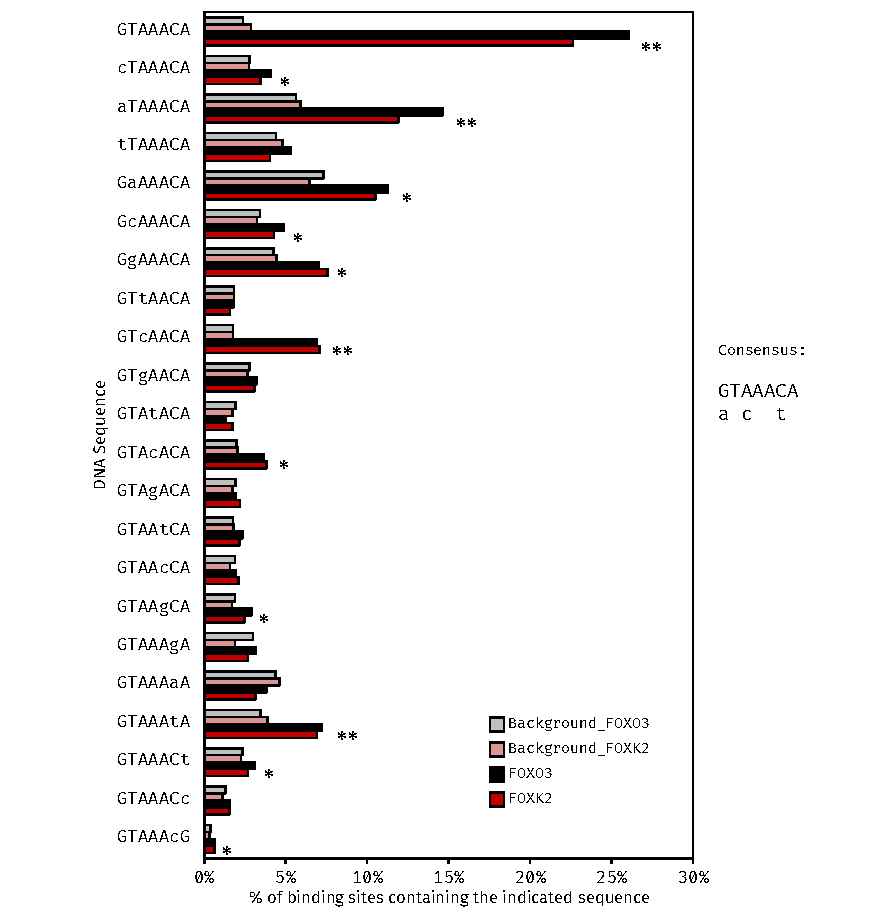
\includegraphics[width=0.9\textwidth]{chapter3/figures_foxo3/fig45.pdf}
    \caption[Binding specificities of FOXK2 and FOXO3 within the Forkhead core consensus]{\textbf{Binding specificities of FOXK2 and FOXO3 within the Forkhead core consensus.} The occurrence of each indicated heptameric sequences within the 200 bp regions centred on the FOXK2 or FOXO3 summit. * represents $P<0.0001$ by a chi-square test. ** represents $P<0.0001$ and indicates the sequences that have 2-fold enrichment of occurrence over the background. The background sequences were randomly chosen from the genome based on the genomic distribution of FOXK2 and FOXO3 binding peaks respectively. The summarised consensus is shown at the right.}
    \label{fig:fig45}
\end{figure}

Given the similarity and the difference of the motifs enriched within FOXK2 and FOXO3 peaks, it is reasonable to speculate that FOXK2 and FOXO3 have a related but different specificity towards the Forkhead consensus, and their interactions with different transcription factors might also contribute to their redundant and specific binding. To test these hypotheses, we first investigated whether FOXK2 and FOXO3 have different specificities to the nucleotides within and flanking the Forkhead core consensus. To this end, we checked the occurrences of a series of heptameric sequences within the 200 bp regions centred on the summit of FOXK2 or FOXO3 bound regions based on the core GTAAACA sequence with each containing a single nucleotide substitution. Random sets of sequences with the same length and similar genomic distribution were chosen as background sequences for parallel comparison. The most frequent and enriched sequences in both cases were the consensus core GTAAACA, but many other sequences were also overrepresented compared to the background sequence (indicated by * in \textbf{Figure \ref{fig:45}}). If setting a threshold of 2-fold over the background, the enriched sequences contained GTAAACA, ATAAACA, GTCAACA, and GTAAATA, which could be summarised as RTMAAYA. This is extremely similar with the sequence of the previous results from in vitro selection of binding sites of seven Forkhead proteins (\cite{pierrou1994cloning}). More importantly, the frequency of each heptameric was nearly identical within FOXK2 peaks and FOXO3 peaks (\textbf{Figure \ref{fig:fig45}}). In addition, the occurrences of GTAAACA, ATAAACA, GTCAACA and GTAAATA were also very similar among the FOXK2-specific peaks, the shared peaks, and the FOXO3-specific peaks (data not shown). These findings indicate that FOXK2 and FOXO3 have very similar binding specificities towards the sequences within the Forkhead core consensus.

Having checked the preferences of FOXK2 and FOXO3 within the Forkhead core sequence, we next investigated whether the DNA sequence flanking the core would influence FOXK2 or FOXO3 binding. To gain an insight into the binding specificities of FOXK2 and FOXO3 at the flanking regions, 5 base pairs upstream and downstream of the GTAAACA core sequence were extracted from the ChIP-seq binding regions, and the frequencies of A, C, G and T nucleotide were counted at each flanking position (\textbf{Figure \ref{fig:fig46}A}). As a comparison, 5 base pairs upstream and downstream of the GTAAACA sequence from the whole genome were also extracted as background.

\begin{figure}[!h]
    \centering
    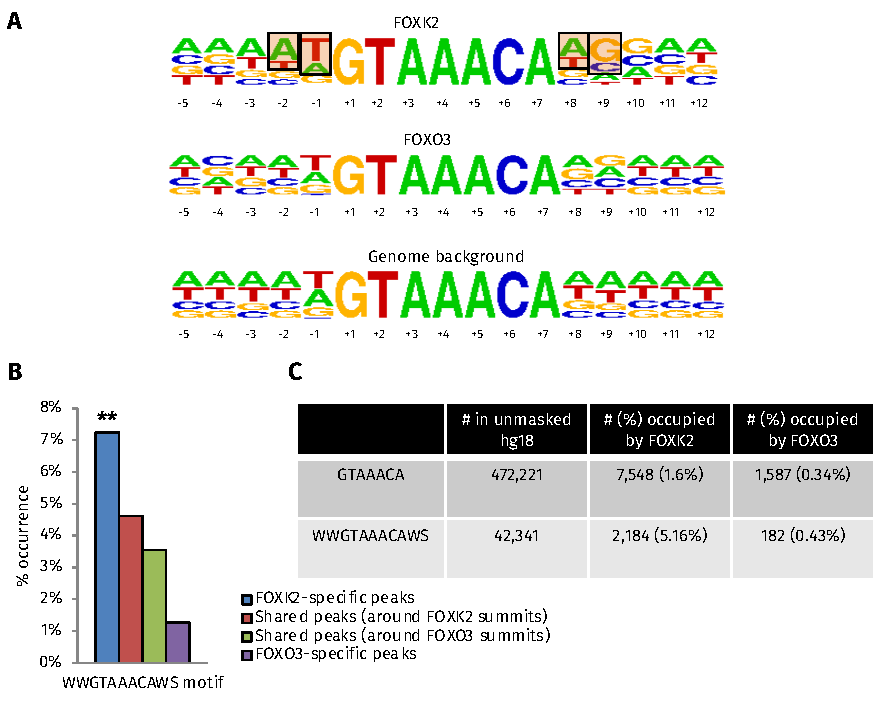
\includegraphics[width=0.9\textwidth]{chapter3/figures_foxo3/fig46.pdf}
    \caption[Nucleotides flanking the core sequence better discriminate FOXK2 from FOXO3 binding]{\textbf{Nucleotides flanking the core sequence better discriminate FOXK2 from FOXO3 binding. (A)} The occurrence of sequences at the flanking regions of the GTAAACA core sequence. 5 bp upstream and 5 bp downstream the core were investigated. Motifs were drawn according to the nucleotide frequency at each position. Yellow rectangles indicate nucleotides whose frequencies are higher than a random distribution using the genome as a background. \textbf{(B)} Percentage of indicated peaks ($\pm$ 200 bp from the summit) that contain the motif WWGTAAACAWS. ** represents $P<0.0001$, chi-square test. \textbf{(C)} Statistics of the sequences GTAAACA and WWGTAAACAWS in the human genome (unmasked hg18). The numbers of the sequences and the percentage occupied by FOXK2 and FOXO3 are shown.}
    \label{fig:fig46}
\end{figure}

In both cases, there was no strong preference within the flanking regions, but the frequency of some nucleotides at certain positions near the core of FOXK2 was indeed much higher than the genome background (\textbf{Figure \ref{fig:fig46}A}, yellow rectangles). FOXK2 preferred an A/T and T/A at the positions -2 and -1, an A/T and G/C at the positions +8 and +9 positions respectively (\textbf{Figure \ref{fig:fig46}A}, top panel). The frequency of nucleotide occurrence flanking the core was similar to background in the FOXO3 case (\textbf{Figure \ref{fig:fig46}A}, middle panel). These observations indicate that nucleotides flanking the core sequence might partially dictate the binding specificity of FOXK2, but their contribution to FOXO3 specific binding, if any, are marginal. The most frequent FOXK2 binding motif including the nucleotides flanking the core can be summarised as an extended motif: WWGTAAACAWS, which is very similar to the original motif returned from HOMER \textit{de novo} discovery. Indeed, this extended motif was significantly more enriched within FOXK2 specific binding peaks compared to either the shared or the FOXO3-specific peaks (\textbf{Figure \ref{fig:fig46}B}). When looking on a genome-wide scale, only 1.6\% of total GTAAACA in the human genome was occupied by FOXK2, but 5.16\% of total WWGTAAACAWS was bound by FOXK2 (\textbf{Figure \ref{fig:fig46}C}). In contrast, 0.34\% of total GTAAACA in the whole genome was occupied by FOXO3, and the percentage (0.43\%) of WWGTAAACAWS bound by FOXO3 was only slightly higher than that of the core GTAAACA motif (\textbf{Figure \ref{fig:fig46}C}). This implies that FOXK2, but not FOXO3, possesses some sequence preference at the regions flanking the Forkhead core consensus.

The sequence analysis within the FOXK2 and FOXO3 binding sites suggest that nucleotides flanking the Forkhead core consensus play some role in the DNA binding of FOXK2. However, \textit{in vivo} binding does not necessarily reflect the intrinsic specificity of a factor due to the presence of many other DNA binding factors in the nucleus. To test whether the sequences in the flanking regions of the Forkhead consensus affect the intrinsic affinity of FOXK2 to DNA, \textit{in vitro} competition EMSAs were performed. The DNA sequence from the \textit{MMP9} locus where FOXK2 binds was used as a binding site. The wild type binding site contains the sequence TT\underline{GTAAACA}AG (\textbf{Figure \ref{fig:fig47}A}). The mutant binding sites also contain the Forkhead core consensus GTAAACA, but the nucleotides at either 5' or 3' to the core consensus were mutated (\textbf{Figure \ref{fig:fig47}A}). We tested the abilities of these unlabelled sequences to compete with the \sus{32}P-labelled wild-type sequence. Reduced binding between FOXK2 and the \sus{32}P-labelled wild-type sequence was observed with the addition of increasing concentrations of both the wild-type and the mutant unlabelled sequences (\textbf{Figure \ref{fig:fig47}B}, lanes 3-14), indicating FOXK2 can bind to both the wild-type and the mutant sequences. However, neither of the mutant probes was as efficient as the wild- type probe to compete for the binding of FOXK2 (\textbf{Figure \ref{fig:fig47}B}, compare lanes 3, 7 and 11). This suggests that nucleotides flanking the Forkhead core consensus indeed affect the intrinsic FOXK2 DNA binding, although the difference between the WT sequence and the Mut2 sequence failed to reach statistical significance when relatively low concentrations of unlabelled sequences were added (\textbf{Figure \ref{fig:fig47}C}). Mutations of nucleotides at the 5' flank of the core consensus had greater effect than the mutations at the 3' flank of the core consensus (\textbf{Figure \ref{fig:fig47}B}, compare lanes 9 and 13), indicating sequences at the 5' flank of the core consensus contribute relatively more to the FOXK2 DNA binding.

Interestingly, the competition EMSA results were consistent with the crystal structure of the DNA-binding domain of FOXK2 with DNA (\cite{tsai2006crystal}). The DNA sequence used in the structure of FOXK2 DBD-DNA complex was 5'-TGTT\underline{GTAAA}- \underline{CA}ATACA-3'. Base-specific contacts were observed not only within the GTAAACA core consensus, but also at the TpT dinucleotides upstream the consensus and ApT dinucleotides downstream the consensus, indicating the specific interactions between FOXK2 and the DNA exist at the flanking regions (\cite{tsai2006crystal}). In addition, such specific interactions were not seen in the structures of FOXO3 DBD or FOXA3 DBD with DNA (\cite{tsai2006crystal,clark1993co-crystal}).

\begin{figure}[!h]
    \centering
    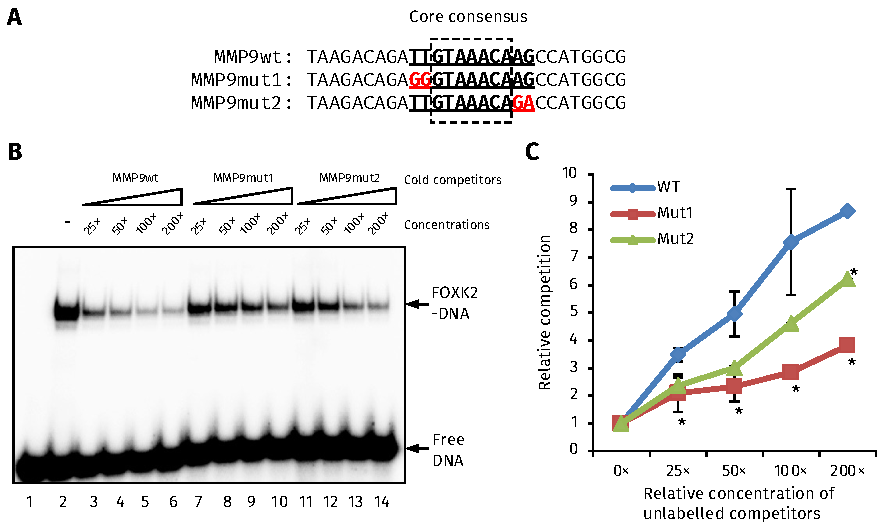
\includegraphics[width=0.9\textwidth]{chapter3/figures_foxo3/fig47.pdf}
    \caption[Competition EMSA experiments to assess the effect of the nucleotides flanking the Forkhead consensus on FOXK2 DNA binding]{\textbf{Competition EMSA experiments to assess the effect of the nucleotides flanking the Forkhead consensus on FOXK2 DNA binding. (A)} DNA sequences used in the experiments. The Forkhead core consensus from the FOXK2 binding region in the \textit{MMP9} regulatory region is highlighted, and the mutations are shown in red colours. \textbf{(B)} Competition EMSA experiments to test the contribution of the nucleotides flanking the Forkhead consensus to the intrinsic binding affinity of FOXK2. Experiments were performed using 90 nM of purified FOXK2 DNA-binding domain and the \sus{32}P-labelled wild-type sequence, together with varying concentrations of the indicated unlabelled binding sites. The unlabelled competitors and their concentrations relative to the \sus{32}P-labelled binding site (taken as 1$\times$) are indicated above the gel. No protein was added at the lane 1. No cold competitors were added at the lane 2. \textbf{(C)} Relative quantification of the FOXK2- DNA complex in \textbf{(B)}. The intensity of FOXK2-DNA complex in the absence of competitors was taken as 1. The reciprocals of the intensity of FOXK2-DNA complex were plotted against the relative concentrations of the unlabelled competitors. The error bars represent the standard deviations from two independent experiments. * and ** represent $p<0.05$ and $p<0.01$ respectively.}
    \label{fig:fig47}
\end{figure}

In summary, both FOXK2 and FOXO3 bind to the consensus RTMAAYA, with GTAAACA being the most overrepresented binding sequence in the cistrome of both factors. Generally, FOXK2 and FOXO3 do not have discernible specificities towards the core sequence. However, FOXK2 has some sequence preference at the regions flanking the core sequence, and the extended motif of FOXK2 can be summarised as WWGTAAACAWS. Indeed, nucleotides at the flanking regions are important for the intrinsic DNA binding of FOXK2, since mutations at the nucleotides flanking the Forkhead consensus reduce the DNA binding of FOXK2 \textit{in vitro}. Similar experiments need to be done in future using the FOXO3 DNA-binding domain to investigate whether FOXO3 also has sequence preferences at the flanking regions of the Forkhead core consensus.

\subsection{Different transcription factors might contribute to the specific binding of FOXK2 and FOXO3}

After exploring the specificities of FOXK2 and FOXO3 towards the Forkhead consensus, we next performed a detailed analysis on other motifs identified from the ChIP-seq derived peaks of FOXK2 and FOXO3, and further investigated the potential roles of other transcription factors on FOXK2 and FOXO3 binding specificities.

To this end, we first checked the enrichment of different motifs discovered from the FOXK2 and FOXO3 cistromes (\textbf{Figure \ref{fig:fig44}A}) within the top 1000 peaks (ranked by the FDR and fold enrichment from MACS) from FOXK2-specific, shared, and FOXO3-specific binding regions respectively. Consistent with previous results, the Forkhead core consensus GTAAACA motif was enriched in all shared and specific peaks of FOXK2 and FOXO3, but the extended Forkhead motif WWGTAAACAWS was more enriched in regions where FOXK2 binds (\textbf{Figure \ref{fig:fig48}A}). The enrichment of the AP1 motif was relatively similar across different classes of peaks (\textbf{Figure \ref{fig:fig48}A}). However, the TEAD motif, the RUNX motif and the CTCF motif were more enriched where FOXK2 binds, and the ETS motif was more enriched where there is FOXO3 binding (\textbf{Figure \ref{fig:fig48}A}).

The differential enrichment of motifs within the specific binding sites of FOXK2 and FOXO3 respectively suggest that they can co-bind with various transcription factors. However, the presence of a motif does not predict the binding of a transcription factor. This is especially the case when it comes to the CTCF transcription factors, where there is some dispute on its binding consensus (\cite{cuddapah2009global,martin2011genome-wide,rhee2011comprehensive}). Therefore, to gain an insight into the potential co-binding of FOXO3/FOXK2 and other transcription factors, and more importantly, to investigate whether the co-binding potentially influences their specificities, we looked into multiple ChIP-seq data sets including ETS1 and RUNX1/3 in Jurkat T cells (\cite{hollenhorst2009dna}), and CTCF in K562 cells (\cite{ernst2011mapping}; and ENCODE project), which might contribute to their binding events.

\begin{figure}[!ht]
    \centering
    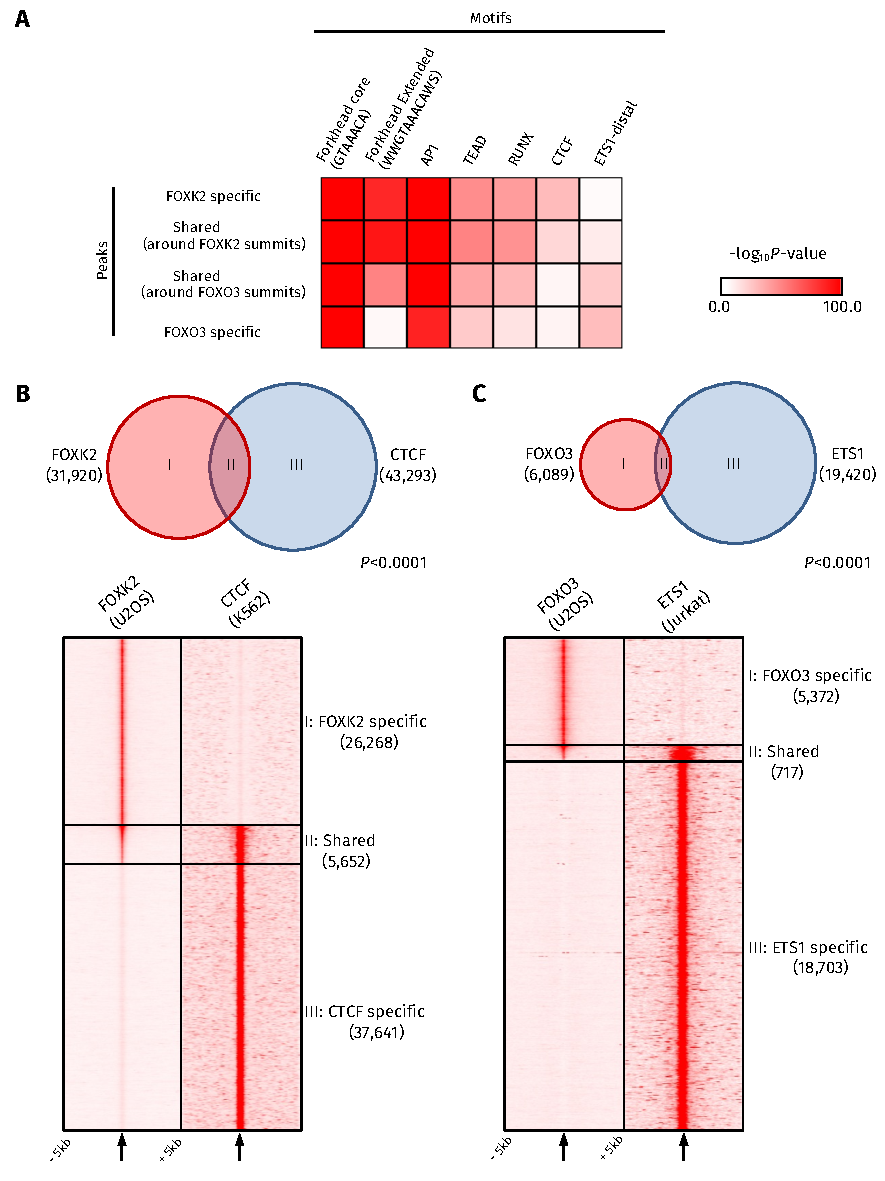
\includegraphics[width=0.9\textwidth]{chapter3/figures_foxo3/fig48.pdf}
    \caption[Co-binding of FOXK2 and FOXO3 with other transcription factors]{\textbf{Co-binding of FOXK2 and FOXO3 with other transcription factors. (A)} The enrichment of each motif within  $\pm$200 bp of the summits from the indicated peaks (top 1000 peaks, ranked by the FDR and fold enrichment). The heatmap was generated using the -$log_{10}$P-value of the indicated motifs calculated by a hypergeometric distribution. \textbf{(B) Top,} a Venn diagram showing the overlap between the FOXK2 peaks and the CTCF peaks. Numbers of total FOXK2 peaks and CTCF peaks were indicated. I, II, and III represent FOXK2-specific peaks, shared peaks and the CTCF-specific peaks respectively. The P-value of the overlap was calculated by a chi-square test. \textbf{Bottom,} heatmap of tag density profiles of FOXK2 and CTCF around the three classes of peaks shown at the top. Numbers of peaks within each class are indicated. Tags were calculated in every 50 bp bin, and the density profiles were normalised to tags per 10 million total reads per bin. The middle point of each panel (indicated by small arrows below) represents the summit of the FOXK2 or CTCF peak. 5 kb upstream and 5 kb downstream around the summit were plotted. Peaks in class I and II were aligned by the FOXK2 summits, and peaks in class III were aligned by the CTCF summits. \textbf{(C)} The same analysis as \textbf{(B)} with the FOXO3 and ETS1 ChIP-seq data.}
    \label{fig:fig48}
\end{figure}

The overlap between RUNX1/3 with FOXK2 and FOXO3 was only marginal (data not shown), indicating that they do not tend to bind to the same locations. The cell type difference might be a reason, and it is also possible that FOXK2 co-localises with a different RUNX factor like RUNX2. Significant overlaps between FOXK2 and CTCF, and between FOXO3 and ETS1 were observed (\textbf{Figure \ref{fig:fig48}B} and \textbf{(C)}). Consistent with the motif enrichment analysis, the overlap between FOXK2 and CTCF was more significant than the overlap between FOXO3 and CTCF ($P<0.0001$, chi-square test), and the overlap between FOXO3 and ETS1 was more significant than that between FOXK2 and ETS1 ($P<0.0001$, chi-square test). Furthermore, detailed analysis on tag density profiles on the overlapping peaks of these factors demonstrated that the reads of CTCF and ETS1 were nicely clustered around the summit of FOXK2 and FOXO3 respectively, indicating that CTCF and ETS1, indeed, bind to the same locations or in close proximity to FOXK2 and FOXO3 respectively (\textbf{Figure \ref{fig:fig48}B} and \textbf{(C)}, class II peaks). These findings indicate that CTCF and ETS1 might contribute to FOXK2 and FOXO3 specific binding as well as their biological functions respectively.

In summary, the possibilities that other transcription factors contribute to the specific binding events of FOXK2 and FOXO3 have been explored through bioinformatic analyses. The CTCF motif was more enriched within the FOXK2 cistrome, while the ETS1 motif was more enriched within the FOXO3 cistrome. Co-localisation of binding events between FOXK2 and CTCF, and between FOXO3 and ETS1 were observed, indicating that potential interactions with other transcription factors might partially contribute to FOXK2 and FOXO3 binding specificity and/or help specify their transcriptional regulatory activities.

\subsection{The enigmatic relationship between FOXK2 and FOXO3 binding}

Having characterised the specific and the shared binding events of FOXK2 and FOXO3, we next investigated the relationship of the DNA binding between these two factors.

Since FOXO3 and FOXK2 belong to the same family and possess many shared binding events, one would expect that they compete for binding sites within those shared peaks, which happens when different factors bind to the same sites (\cite{pierce2003sum1,zhou2011integrated}). On the other hand, the fact that binding signals of both FOXK2 and FOXO3 are generally higher around the shared peaks indicates that an assisted binding mechanism is also possible. Indeed, Forkhead transcription factors, like FOXA1, have been demonstrated as pioneer priming factors for several nuclear receptors like ER (\cite{hurtado2011foxa1}) and AR (\cite{wang2011reprogramming}), though the role of FOXA1 in the latter case is more complicated. FOXK2 is constantly nuclear (\cite{marais2010cell}), but FOXO3 is sequestered in the cytoplasm under normal condition and goes into the nucleus when the PI3K/AKT signalling is inhibited. This resembles the behaviour of those nuclear receptors which also translocate to the nucleus upon receiving a signal through ligand binding. Therefore, it is also tempting to speculate that FOXK2, which is constantly nuclear, acts as a pioneer priming factor for FOXO3 in U2OS cells.

\begin{figure}[!ht]
    \centering
    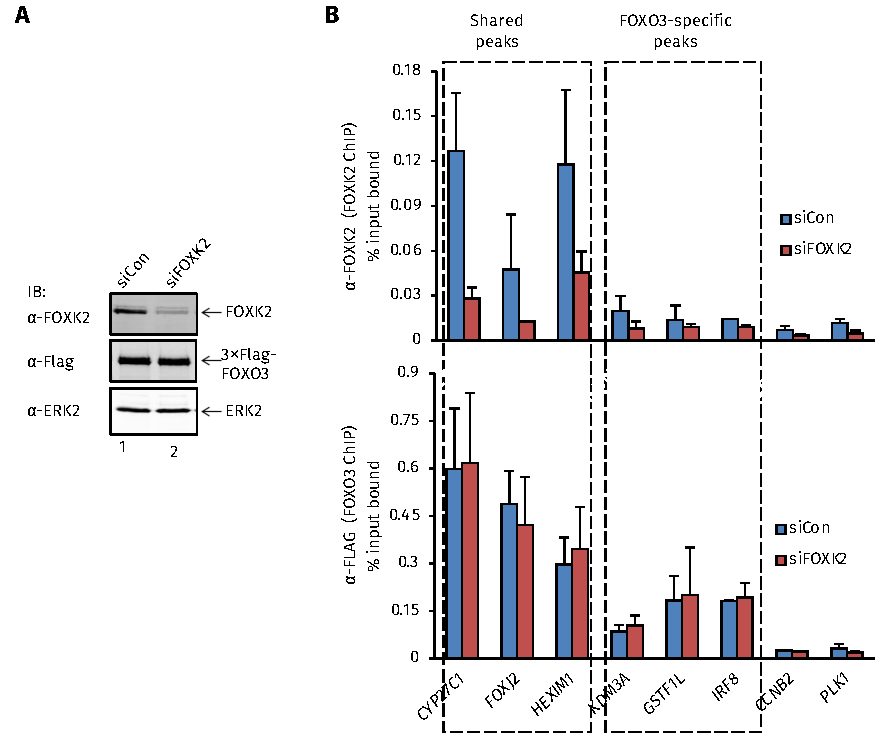
\includegraphics[width=0.9\textwidth]{chapter3/figures_foxo3/fig49.pdf}
    \caption[Knockdown of FOXK2 has little effect on the DNA binding of FOXO3]{\textbf{Knockdown of FOXK2 has little effect on the DNA binding of FOXO3. (A)} Western blot analysis showing the endogenous FOXK2 protein level after the depletion of FOXK2. The U2OS-FOXO3 stable cell line was transfected with a non-targeting siRNA or a siRNA against FOXK2. Protein expression levels were examined by immunoblotting (IB) with the indicated antibodies. \textbf{(B)} The U2OS-FOXO3 stable cell line was treated with doxycycline to induce the expression of the FLAG-tagged FOXO3 transgene, and were transfected with 20 nM non-targeting siRNA or siRNA against FOXK2. LY294002 were added to cells 2 hours before crosslinking the cells. ChIP experiments were performed either using a FOXK2 antibody (top) or a FLAG antibody (bottom). The shared regions and the FOXO3-specific regions are indicated by dashed rectangles. The error bars represent the standard deviations from two independent experiments.}
    \label{fig:fig49}
\end{figure}

To test whether FOXK2 competes with or primes for the FOXO3 binding, 3$\times$FLAG- FOXO3 was induced to the level comparable to the endogenous FOXO3 by adding doxycycline (\textbf{Figure \ref{fig:fig11}B}, lane 3), and FOXO3 was activated by the treatment of cells with LY294002. ChIP experiments were performed after the knockdown of FOXK2 by siRNA transfection, and the DNA binding was measured by locus-specific qPCR. Six peaks from the ChIP-seq data, including three shared peaks and three FOXO3 specific peaks, were tested. The \textit{CCNB2} and the \textit{PLK1} loci were used as negative control regions. Western blot analyses showed that the FOXK2 protein level was significantly reduced after the knockdown of FOXK2, although there was still some detectable FOXK2 protein (\textbf{Figure \ref{fig:fig49}A}). The expression of 3$\times$FLAG-FOXO3 was unaffected by the treatment of the FOXK2 siRNA (\textbf{Figure \ref{fig:fig49}A}). After the depletion of FOXK2, either increased (indicating competition with FOXK2) or decreased (indicating primed by FOXK2) FOXO3 binding was expected. The FOXK2 binding signals were reduced at the shared binding regions after the treatment with siFOXK2, and its binding levels at the FOXO3-specific regions were comparable to the background (\textbf{Figure \ref{fig:fig49}B}, top panel). However, the FOXO3 binding signals were hardly affected by the FOXK2 knockdown (\textbf{Figure \ref{fig:fig49}B}, bottom panel). It seems that under current experimental conditions, neither competitive nor cooperative binding between FOXK2 and FOXO3 could be detected.

To further investigate the relationship between FOXK2 and FOXO3 DNA binding, FOXK2 ChIP experiments were performed after the activation of the endogenous FOXO3 by the treatment of LY294002. Similarly, no discernible changes of FOXK2 binding could be observed on the tested regions (\textbf{Figure \ref{fig:fig50}A}). However, addition of LY294002 will inhibit PI3K/ATK signalling, which might also affect FOXK2 DNA binding. Since previous immunofluorescence experiments demonstrate that some FOXO3 protein is located in the nucleus under normal cell culture condition (\textbf{Figure \ref{fig:fig11}C}), we just forced the overexpression of FOXO3 to increase its nuclear concentration by simply adding a high concentration of doxycycline under normal cell culture condition (with FCS, without LY294002) to circumvent any possible effects of LY294002 on FOXK2 DNA binding. Western blot analyses showed that the expression of 3$\times$FLAG-FOXO3 was significantly elevated after the addition of a high concentration of doxycycline (\textbf{Figure \ref{fig:fig50}B}). More importantly, the overexpression of FOXO3 resulted in an increased DNA binding on all tested regions even without LY294002 treatment (\textbf{Figure \ref{fig:fig50}B}, top panel). However, similar to previous results, the changes of FOXK2 binding were only marginal, even though the binding of FOXO3 was significantly increased at the same region (\textbf{Figure \ref{fig:fig50}B}, bottom panel).

\begin{figure}[!h]
    \centering
    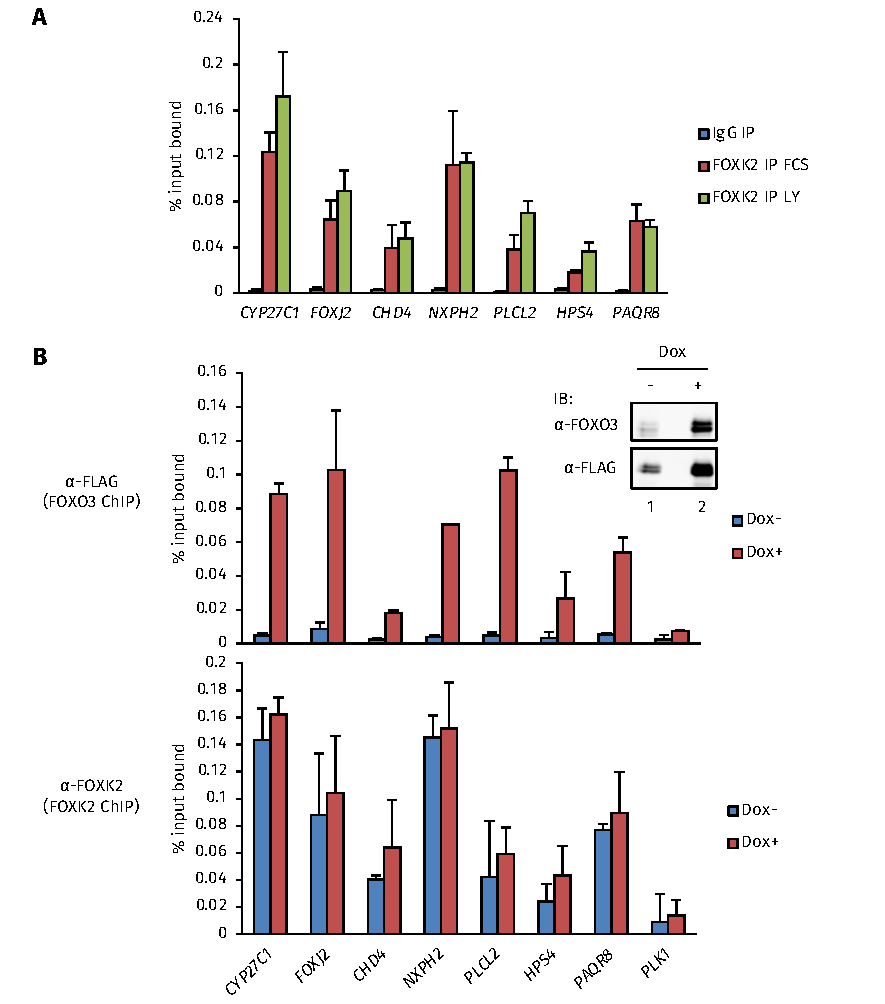
\includegraphics[width=0.9\textwidth]{chapter3/figures_foxo3/fig50.pdf}
    \caption[Changes of FOXO3 binding do not significantly affect FOXK2 binding]{\textbf{Changes of FOXO3 binding do not significantly affect FOXK2 binding. (A)} FOXK2 ChIP experiments with or without the treatment with LY294002. U2OS cells were cultured under normal condition (FCS) or treated with LY294002 (LY) for 2 hours before performing the experiments. ChIP was done using a FOXK2 antibody. A non-specific IgG antibody was also included as a control. The error bar represents the standard deviation from two independent experiments. \textbf{(B)} FOXO3 and FOXK2 ChIP with or without FOXO3 overexpression. The U2OS-FOXO3 stable cell line was either untreated (Dox-) or treated with 1 $\mu$g/mL doxycycline (Dox+) for 24 hours before experiments. ChIP experiments were done using a FLAG antibody (top) or a FOXK2 antibody (bottom). The \textit{PLK1} locus was used as a negative control region. The error bar represents the standard deviation from two independent experiments. Western blot analysis showing the overexpression of the FLAG-tagged FOXO3 transgene after the addition of doxycycline is shown at the top right corner. The U2OS-FOXO3 stable cell line was treated with 1 $\mu$g/mL doxycycline for 24 hours. Protein expression levels were examined by immunoblotting (IB) with the indicated antibodies.}
    \label{fig:fig50}
\end{figure}

The observations that changes of FOXK2 binding does not affect the FOXO3 binding and vice versa suggest that their DNA binding events are independent of each other. It is likely that FOXK2 and FOXO3 bind to the same site but in different cells. If this is the case, changes of the binding of one factor will only affect the binding of the other factor in a subfraction of the cells, which might not be able to be detected by our ChIP experiments. It is also possible that FOXK2 and FOXO3 bind to the same region but at different sites, which cannot be discriminated by the resolution of sonication-based ChIP-seq method that we use. However, it is also likely that current ChIP experiments which analyse the steady-state \textit{in vivo} protein-DNA interactions are unable to detect the subtle dynamic changes of DNA-binding of FOXK2 and FOXO3.

To gain a preliminary idea of whether FOXK2 and FOXO3 bind to different sites or not, we looked into the redundant peaks and analysed the distance between the summits of FOXK2 and FOXO3. The majority of FOXO3 and FOXK2 summits were within 160 bp, though a small proportion of their summits were relatively far away from each other (\textbf{Figure \ref{fig:fig51}A}). This indicates that the exact binding sites of FOXK2 and FOXO3 are close, if not the same. Since the heptameric sequences GTAAACA, ATAAACA, GTCAACA and GTAAATA (hereafter known as FOXK2/O3 motifs) are the most enriched sequences within the FOXK2 and FOXO3 cistromes (\textbf{Figure \ref{fig:fig45}}), they are presumably the direct binding sequences of FOXK2 and FOXO3. Within the shared peaks, \textasciitilde 58\% of them contain at least one FOXK2/O3 motif. Among these peaks, most only contain one site of FOXK2/O3 motif per peak within the 200-bp region around the FOXK2 summit (\textbf{Figure \ref{fig:fig51}B}). The analysis on the FOXO3 summits within the shared peaks yielded the same result (data not shown). These findings indicate that in most cases, there is only one site available for Forkhead proteins to bind at the shared peaks. Therefore, based on the proximity of their summit and the occurrence of the FOXK2/O3 motifs within the peaks, the favourable extrapolation from these results would be that the binding of FOXK2 and the binding FOXO3 are likely mutually exclusive.

\begin{figure}[!h]
    \centering
    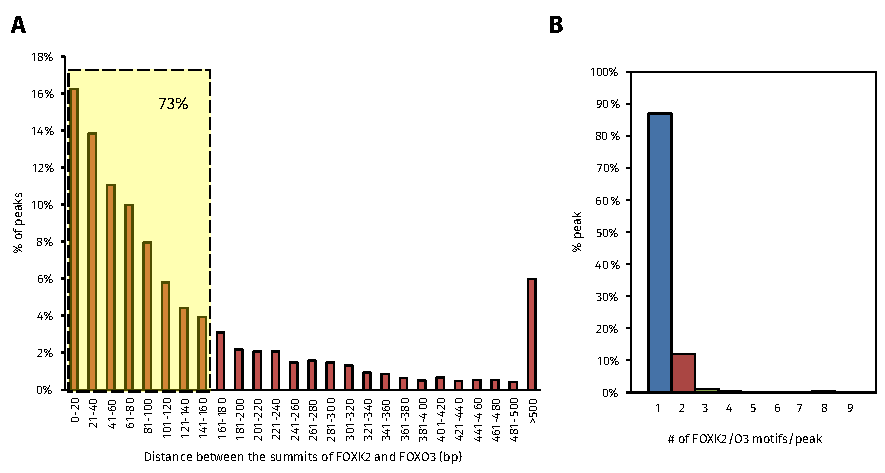
\includegraphics[width=0.9\textwidth]{chapter3/figures_foxo3/fig51.pdf}
    \caption[Distance between FOXK2 and FOXO3 summits and the occurrence of the FOXK2/O3 motifs within the shared peaks]{\textbf{Distance between FOXK2 and FOXO3 summits and the occurrence of the FOXK2/O3 motifs within the shared peaks. (A)} Histogram showing the distance between the FOXK2 and FOXO3 summits. The shared peaks coordinates were extracted, and the distance of the FOXK2 and FOXO3 summits within each peak was calculated. \textbf{(B)} Histogram showing that the frequency of occurrence of FOXK2/O3 motifs (GTAAACA, ATAAACA, GTCAACA and GTAAATA) within the shared peaks. Sequences from the shared peaks ($\pm$ 200 bp from the FOXK2 summits) were extracted, and the occurrence of FOXK2/O3 motifs was counted per peak.}
    \label{fig:fig51}
\end{figure}

In summary, changes of FOXK2 binding do not seem to affect FOXO3 binding, and increased FOXO3 binding cannot displace FOXK2 from the chromatin. Bioinformatic analyses show that the summits of FOXK2 and FOXO3 are very close, and most of their shared peaks only contain one available Forkhead binding site (FOXK2/O3 motifs) per peak, indicating that FOXK2 and FOXO3 are likely to bind to the same site. Therefore, the question still remains: given that FOXK2 and FOXO3 cannot bind to the same site together, what is the relationship between FOXK2 and FOXO3 binding?

\subsection{Summary}

Collectively, the data presented in this section provide a detailed analysis of the FOXO3 ChIP-seq data and a comparison between the FOXO3 and FOXK2 cistromes. Only one experiment was performed for the FOXO3 ChIP-seq, and 6,089 peaks were identified by both MACS and HOMER peak callers.

Many known FOXO3 target genes are successfully detected by our FOXO3 ChIP-seq data. However, a previous study has indicated that FOXO3 binds to the upstream regions of \textit{CCNB1} and \textit{PLK1} promoter, indicating its redundant regulatory role with FOXM1 (\cite{alvarez2001forkhead}). Our FOXO3 ChIP-seq data does not recover such binding events, and ChIP-qPCR results demonstrate that FOXO3 does not bind the core promoters of \textit{CCNB1} and \textit{PLK1} either (\textbf{Figure \ref{fig:fig40}A}). The discrepancy could be due to different experimental conditions: G2-arrested HeLa cells (\cite{alvarez2001forkhead}) and LY294002 treated U2OS cells (this study). A later study has shown that FOXO3 fails to activate a \textit{PLK1} promoter-driven luciferase and forced overexpression of FOXO3 fails to rescue the mitotic defects caused by the loss of FOXM1 (\cite{laoukili2005foxm1}). Therefore, whether FOXO3 really contributes to the execution of mitotic programmes still need further investigation.

Gene ontology analyses recover many known FOXO3 functions like apoptosis, cell cycle arrest, cell differentiation and development. Interestingly, the apoptosis and cell cycle arrest related processes are not enriched when all FOXO3 peaks are analysed. Instead, they are more enriched in the peaks with high FOXO3 binding signals, indicating that high occupancy FOXO3 binding events might reflect the regulation of apoptosis and cell cycle arrest. Novel functions like the regulation of smooth muscle cell migration and blood coagulation are revealed by the FOXO3 ChIP-seq data, suggesting FOXO3 may function as an important regulator within those processes. However, biological functions revealed by our FOXO3 ChIP-seq data must be interpreted with caution, because only one experiment of FOXO3 ChIP-seq was done. Extracting biological functions from a single experiment can be unreliable. In addition, it is interesting to see the differentiation- and development-related terms as well as terms like blood coagulation enriched within the FOXO3 cistrome, considering the U2OS cell line is derived from an osteosarcoma. It is possible that FOXO3 binds to those genes but does not regulate their expression in this cell type. Without downstream experimental validations, no reliable conclusions about the biological functions of FOXO3 can be drawn.

FOXO3 and FOXK2 have both shared and specific peaks, but the majority of FOXO3 binding events are shared with FOXK2. The most overrepresented DNA motifs returned from FOXK2 or FOXO3 ChIP-seq derived peaks are both Forkhead like responsive elements containing the core GTAAACA. Certain substitutions within the core sequence are tolerable, and the consensus can be summarised as RTMAAYA, with GTAAACA being the most frequent motif in both cases. FOXK2 and FOXO3 possess the same sequence preference within the core consensus, but some nucleotides flanking the core consensus are more overrepresented within the FOXK2 peaks, compared to the FOXO3 peaks and the genome background. This preference of FOXK2 towards the flanking nucleotides can be summarised as an extended motif WWGTAAACAWS, and the \textit{in vitro} competition EMSA experiments suggest that mutations of the nucleotides flanking the Forkhead consensus indeed affect the DNA binding of FOXK2. Of note, only nucleotides flanking the most frequent heptameric sequence GTAAACA were investigated in this study. It is possible that when bound to a different core consensus (\textit{e.g.} GTCAACA), FOXK2 or FOXO3 has different preferences at the flanking region. Further experiments need to be done to address this issue.

Besides the Forkhead like motif, several responsive elements that are recognised by other transcription factors are also enriched within the FOXK2 and FOXO3 ChIP-seq derived peaks, and comparisons with other transcription factor ChIP-seq datasets indicate FOXK2 and FOXO3 might cooperate with those transcription factors to regulate gene expression. The CTCF and the ETS1-distal motifs were differentially enriched within the FOXK2 and FOXO3 cistromes respectively. Co-localisation of the binding events between the insulator CTCF and FOXK2, and between ETS1 and FOXO3 were observed, suggesting that CTCF might contribute to FOXK2 specific binding events, and ETS1 might help FOXO3 gain its own specific binding peaks. The different TF-TF cooperation might also help FOXK2 and FOXO3 gain their specific biological functions. However, since the ChIP-seq data sets are from different labs and different cell lines, the comparison performed in this section is just a reference. Without further wet lab experimental validation, no firm conclusions can be drawn.

On the other hand, preliminary data suggests that some cooperation of binding events might exist. For example, our recent study of FOXK2 has revealed many FOXK2 binding proteins including SIN3A and SET (Z.Ji, unpublished data), both of which have been shown to interact with CTCF (\cite{lutz2000transcriptional,yusufzai2004ctcf}). In addition, another CTCF interaction partner YY1 can form a ternary complex with BAP1 and HCF1 (\cite{yu2010the}), both of which interact with FOXK2 (Z.Ji unpublished data). Interestingly, another Forkhead transcription factor FOXA1 is shown to have a subset of binding events that overlap with CTCF (\cite{ross-innes2011a}).

The distance of FOXK2 and FOXO3 summits is close, and the majority of the shared peaks only contain one FOXK2/O3 motif. Since no evidence suggests the FOXK2 physically interacts with FOXO3, hence it is reasonable to speculate that the binding of FOXK2 and FOXO3 at their shared peaks are mutually exclusive (\textit{i.e.} binding at different cells). However, ChIP results indicate that the change of FOXK2 binding does not have any detectable effects on FOXO3 binding within their shared peaks and vice versa. This leaves an interesting question of how they bind to their shared peaks. These two proteins might utilise some novel mechanisms to achieve their binding events at the shared peaks. Further investigation need to be done to address this question (see \textbf{Chapter \ref{ch:conclusions}}).